\documentclass[a4paper]{scrartcl}
\usepackage[utf8]{inputenc}
\usepackage[T1]{fontenc}
\usepackage{amsmath,enumerate}
\usepackage{amsfonts}
\usepackage{graphicx}
\usepackage{multicol}
\usepackage{subfig}
\usepackage{float}
\usepackage{listings}
\lstset{language=sql,basicstyle=\small,keywordstyle=\ttfamily,morekeywords={REFERENCES,DEFERRED}}
\usepackage{tabularx}
\PassOptionsToPackage{hyphens}{url}\usepackage{hyperref}
\usepackage{enumitem}

\usepackage{scrpage2}
\pagestyle{scrheadings}

\newcommand{\ul}[1]{\underline{#1}}
\newcommand{\ra}{\rightarrow}
\newcommand{\R}{\ensuremath{\mathcal{R}}}

\newtheorem{ex}{Exercise}
\newenvironment{exercise}[2]%
   {\def\tmp{}%
    \ifx\points\tmp
      \begin{ex}
    \else
      \def\tmp{1}%
      \begin{ex}[#1][#2 points\ifx\points\tmp\else \fi]
    \fi
    \normalfont
   }%
   {\end{ex} %
   }



\title{Exercise Sheet 2, 2020}
\subtitle{6.0 VU Advanced Database Systems}
\author{}

\automark{section}
\ohead{\pagemark}
\makeatletter
\chead{ADBS 2020 -- \@author}
\makeatother
\cfoot{}

\begin{document}
\maketitle





\begin{exercise}{Costs of MapReduce}{1}
\begin{enumerate}[label=\alph*)]
	\item \label{1a} The purpose of a combiner is to do some reduce functionality already after the mapping phase. Since we do not use them in this case, all reduce functionality needs to be implemented in the reducers.
	
	Each reduce task receives a different (key,value list) pair. So there is likely to be a skewed processing time in the reduce tasks, as the keys (i.e. words) will certainly differ in the length of their value lists.
	
	What we do not know, though, is how the reduce tasks are distributed to the specific reducers (we use "some number" of reducers). The lower the number of reducers used, the less will be the skew with respect to the reducers.
	\item The skew is unlikely to be significant, since the number of keys (i.e. words) will be significantly larger than the number of reduce tasks. On the other hand, when 10,000 reduce tasks are used, there will probably emerge a significant skew. Again, similar to \ref{1a}, if we are concerned with the skew of the reducers, this will depend on how many reducers we use.
	\item Adding a combiner after the mapper will not affect the skew, if we assume that the relief provided by the combiner is the same (or nearly the same) for all reduce tasks. If that is not the case, i.e. if the combiner provides relief proportional to the lengths of the value lists, then the skew will be severly reduced.
	\item Per se, the communication cost will not increase  by increasing the number of reduce tasks. However, it might be sensible to assume that we also increase the number of reducers proportionally to the number of reduce tasks. In this case, the communication cost will certainly increase. 
	
	Since the replication rate depends on the mappers but not the reducers, it would not change in this scenario. Also, since the reducer size is the maximum value list length of individual keys, it does not change in this scenario.
\end{enumerate}
\end{exercise}


\begin{exercise}{Relational Operations}{2}
\begin{enumerate}[label=\alph*)]
	\item 
	\begin{itemize}
		\item Map function:
		\begin{itemize}
			\item output ($r$;"R") $\forall r \in R$ and ($s$;"S") $\forall s \in S$.
		\end{itemize}
		\item Reduce function:
		\begin{itemize}
			\item Input is ($t$;[$x_1 \dots x_n$]) where $x_i$ is either "R" or "S".
			\item Counts the occurences of "R" $|x_R|$ and the occurences of "S" $|x_S|$.
			\item Output ($t$,$t$) $\max(|x_R|-|x_S|, 0)$ times.
		\end{itemize}
		\item Communication cost: since the replication rate is 1 and since there is no combiner, the communication cost is $|R| + |S|$.
	\end{itemize}
	\item
		\begin{itemize}
		\item Map function:
		\begin{itemize}
			\item output (key=($r.b,r.c$);value=("R", $r.a$)) $\forall r \in R$ and (key=($s.b,s.c$);value=("S", null)) $\forall s \in S$.
		\end{itemize}
		\item Reduce function:
		\begin{itemize}
			\item Input is (key=($t.b$,$t.c$);values=[$(x_1, y_1) \dots (x_n, y_n)$]) where $x_i$ is either "R" or "S" and $y_i$ is $t.a$ if $x_i=$"R" and null otherwise.
			\item If $\not\exists x_i$ for which $x_i=$"S" then output ($t,t$).
		\end{itemize}
		\item Communication cost: since the replication rate is 1 and since there is no combiner, the communication cost is $|R| + |S|$.
	\end{itemize}
\end{enumerate}
  
\end{exercise}

\begin{exercise}{MapReduce}{4}

\begin{enumerate}[label=\alph*)]
	\item \label{4a} For this job, I have a simple mapper which emits \texttt{(user\_id, brand)} tuples for each input line, provided that the \texttt{event\_type == "purchase"}. As sanity check, I also check that \texttt{brand} and \texttt{product\_id} are non-empty.
	
	The reducer gets a \texttt{(user\_id, [brand])} tuple and emits \texttt{(user\_id, fav\_brand)}, where \texttt{fav\_brand} is the brand with the highest occurrence in \texttt{[brand]}. In cases where multiple brands occur with the same frequency, only the first brand is emitted.
	
	The \texttt{mrjob} package does not produce CSV-formatted output by default. However, the output format can be changed by setting \texttt{OUTPUT\_PROTOCOL} in the job class. I used the \texttt{CsvProtocol} class of the \texttt{mr3px} package.
	
	\item \label{4b} I opted to follow the advice in the assignment sheet and extended the job of \ref{4a} for this task. The job consists of two steps, where the first is similar to \ref{4a}.
	
	The mapper of step one now emits \texttt{(user\_id, (month, brand))} subject to the same conditions as in \ref{4a}. \texttt{month} is calculated using \texttt{event\_time}. Obviously, if this fails for some reason (such as an empty value), nothing is emitted.
	
	The reducer of step one receives \texttt{(user\_id, [(month, brand)])} and checks whether both the month 10 and 11 occur in the tuple list. If this is the case, the most occurring brand is emitted as in \ref{4a}. However, as opposed to \ref{4a}, the most occurring brand is only emitted provided that the occurrences are strictly greater than the occurences of the second-most occurring brand.
	
	The second step uses an inversion mapper and the reducer then simply emits the length of the \texttt{user\_id} value list of each \texttt{brand} key.
	
	In order to operate on both \texttt{2019-Oct.csv} and \texttt{2019-Nov.csv}, I simply call the Python script with both file paths.

	\item 
	\begin{tabular}{c r r r r}
		Job & Map input records & Map output records & Replication rate & Reducer output records\\
		\ref{4a} & 42448765 & 684635 & 1.61\% & 326222 \\
		\ref{4b} step 1 & 109950745 & 684635 & 0.62\% & 40946 \\
		\ref{4b} Step 2 & 40946 & 40946 & 100\% & 866 \\
	\end{tabular}

\end{enumerate}

  
\end{exercise}


\begin{exercise}{Hive Exercise}{4}
\begin{enumerate}[label=\alph*)]
	\item The tables were set up as managed tables and not as external tables. I generally attempted to find fitting types and used \texttt{bigint} for all ids. For the \texttt{ROW TYPE}, I initially wanted to use the OpenCsvSerde. However, I encountered problems with loading the users and posts CSV files using this. Also, it resulted in the tables being forced to use the \texttt{string} type for each column, which I aimed to avoid. Thus, I simply used \texttt{DELIMITED} with a few clauses. I also took care to skip the header.
	
	The only other minor problem were timestamps in the \texttt{postlinks} table. I had to explicitly define the timestamp format in order for the loading to work.
	
	\item The query took 2m1s to complete using the normal tables. I first tried to improve this by using partitions. The only viable candidate in the query for partitions is \texttt{users.reputation}, as this can be easily split on the condition \texttt{u.reputation > 100}.
	
	However, it is not possible to simple define a condition as partition value:
	
	\begin{verbatim}
		insert into table users_partitioned partition (reputation > 100)
		select * from users where reputation > 100;
	\end{verbatim}
	
	Therefore, I used 100 and 101 as partition "markers" and put the tuples for which the condition holds in the 101 partition and the rest in the 100 partition. I also discard unnessecary columns in my code, which makes it easier to read, but obviously does not affect the query. With this optimization, the query runtime is reduced to 1m25s.
	
	Regarding buckets, it quickly became appearant that using them on primary keys does not make any sense, since the key is unique for every tuple. But it could make sense for foreign keys, as they can be the same for multiple tuples. 
	
	\begin{table}[h]
	\begin{tabular}{l r}
	Field & distinct values\\
	\texttt{posts.posttypeid} & 280\\
	\texttt{posts.owneruserid} & 524\\
	\texttt{comments.postid} & 175027\\
	\texttt{postlinks.relatedpostid} & 23388\\
	\end{tabular}
	\label{tab:distinctfk}
	\caption{Distinct values of all columns (except reputation) 
	occuring in the SQL query}
	\end{table}

	As can be seen in \autoref{tab:distinctfk}, \texttt{posts.posttypeid} and \texttt{posts.owneruserid} are plausible candidates for bucketing. Since there is obviously no "multi-level" bucketing in Hive, I tried both columns separately. In theory, one could bucket using both colums, but this would only result in the buckets being created using a hash over the concatenated column values, i.e. not really useful for this query.
	
	When attempting this, I faced the problem that \texttt{posts.owneruserid} and \texttt{posts.posttypeid} are not actually stored as \texttt{bigint}, but have some wrong string values in them. Thus, the bucketing did not really work out.
	
	Looking at the query plan, though, shows that the clustering did not change the query significantly. This is the case, even if \texttt{set hive.optimize.bucketmapjoin = true;} is used. It could be the case that I used the wrong datatypes for clustering. I found out when consulting the documentation\footnote{\url{https://cwiki.apache.org/confluence/display/Hive/LanguageManual+DDL+BucketedTables}} that \texttt{bigint} works differently than \texttt{int} for this sort of task.
	
	Finally, I tried to combine optimization for \texttt{posts.posttypeid} and \texttt{posts.owneruserid} by partitioning using the one and clustering using the other. This turned out to be a bit tricky. I first tried to partition using \texttt{posts.owneruserid}, but for some reason this exceeded the partition limit of 1000. Then, I tried partitioning using \texttt{posts.posttypeid}. This did not work out initially, as somehow \texttt{posts.body} values leaked into the \texttt{posts.posttypeid} column, which made the paths exceed the fs limit. Thus, I use only data where \texttt{posts.posttypeid} is a bigint. Even then, the 
	
In the end, the only viable change is partitioning the \texttt{users} table. The relevant section in the original query plan is shown below:
	
\begin{verbatim}
TableScan
alias: u
filterExpr: (id is not null and (reputation > 100)) (type: boolean)
Statistics: Num rows: 3784748 Data size: 45416976 Basic stats: COMPLETE Column stats: NONE
Filter Operator
predicate: (id is not null and (reputation > 100)) (type: boolean)
Statistics: Num rows: 1261582 Data size: 15138984 Basic stats: COMPLETE Column stats: NONE
Reduce Output Operator
key expressions: id (type: bigint)
sort order: +
Map-reduce partition columns: id (type: bigint)
Statistics: Num rows: 1261582 Data size: 15138984 Basic stats: COMPLETE Column stats: NONE
\end{verbatim}

With partitioning, this changes into a HashTable Sink Operator:

\begin{verbatim}
TableScan
alias: u
filterExpr: (id is not null and (reputation > 100)) (type: boolean)
Statistics: Num rows: 37075 Data size: 5011264 Basic stats: COMPLETE Column stats: NONE
Filter Operator
predicate: id is not null (type: boolean)
Statistics: Num rows: 37075 Data size: 5011264 Basic stats: COMPLETE Column stats: NONE
HashTable Sink Operator
keys:
0 _col14 (type: bigint)
1 id (type: bigint)
\end{verbatim}

\item The original query shown in \autoref{lst:4c.orig} contains two subqueries that render it unable to be executed using Hive:

\begin{enumerate}
\item  A subquery that checks whether a users upvotes are maximal among all users created after a given post
\item A subquery which checks whether another post links to a given post as a related post
\end{enumerate}

\begin{lstlisting}[label=lst:4c.orig, caption=Original Hive query]
SELECT p.id FROM posts p, comments c, users u, badges b
WHERE c.postid=p.id AND u.id=p.owneruserid
AND u.id = b.userid
AND u.upvotes IN (SELECT MAX(upvotes)
FROM users u WHERE u.creationdate > p.creationdate)
AND EXISTS (SELECT 1 FROM postlinks l WHERE l.relatedpostid > p.id)
AND (b.name LIKE 'Research Assistant');
\end{lstlisting}

I eliminated the second subquery by simply including the \texttt{postlinks} table using a join with the condition given in the subquery. Since this only returns tuples that fulfill the condition, I ensure that the condition holds.

The second subquery could be eliminated by joining the \texttt{users} table a second time and finally grouping by \texttt{users.uservotes}. Since \texttt{GROUP BY} supports comparing group keys to aggregate functions of other fields using the \texttt{HAVING} clause, one can compare \texttt{users.uservotes} to \texttt{MAX(users2.uservotes)}.

The resulting query can be seen in \autoref{lst:4c.wosub}.

\begin{lstlisting}[label=lst:4c.wosub, caption=Hive querydraw without subqueries]
SELECT p.id FROM posts p, comments c, users u, users u2, badges b, postlinks l
WHERE c.postid=p.id AND u.id=p.owneruserid
AND u.id = b.userid
AND l.relatedpostid > p.id
AND u2.creationdate > p.creationdate
AND b.name LIKE 'Research Assistant'
group by p.id, u.id, u.upvotes HAVING u.upvotes = MAX(u2.upvotes);
\end{lstlisting}

In the end, I could confirm that the subquery ist executable by Hive and I am also convinced that the originally desired result is returned. However, the performance of the query is abysmal. The runtime is on the order of hours. Thus, I gather there must be some more optimal way to translate this query. I tried using other joins like left (semi) join, but unfortunately, I was not able to come up with a better solution.

\end{enumerate}
\end{exercise}


\begin{exercise}{Spark in Scala}{4}

\begin{enumerate}[label=\alph*)] 
\item I aimed to make use of Spark functions as much as possible. This was relatively straightforward for the first and the last task. Only a single \texttt{collect} action has been used for those.

The median and standard deviation case was a bit more tricky. For the median, I had to use two actions. First, I needed to use \texttt{count} in order to ascertain whether there is an even or an odd number of elements in the array. Then, I had to use \texttt{collect} in order to retrieve the correct median value from the array.

For the standard deviation, I had to resort to three actions. I needed both a \texttt{count} and a \texttt{reduce} action to calculate the average. Then, I used a \texttt{reduce} action to get a sum of squared differences.

\item

\begin{enumerate}[label=Query \arabic*, leftmargin=*] 
	\item The execution plan and the runtime is exactly the same.
\item The conversion is straightforward. Interestingly, although the query plan is exactly the same, the SQL version consistently a bit faster. Using the Spark Web UI (SQL tab) I could find out that both HashAggregate steps are faster for the SQL version. However, this could also be due to an unstable estimate.

\item \label{it:query3} I had to implement the subquery using a pseudo left semi join, as correlated subqueries are not (yet) supported using the DataFrame API\footnote{\url{https://issues.apache.org/jira/browse/SPARK-23945}}. The execution plans differ slightly. The most important difference is that the SQL version uses a left outer join, while the DataFrame API version uses an inner join. In particular, the SQL version has an additional Exchange step after the second HashAggregate step of the oct2 table. In practice, this difference is negligible, as both versions have similar runtimes on average.
\item \label{it:query4} Surprisingly, the execution plans are exactly the same, as are the runtimes. The runtime of the query is significantly higher than the others. I also experienced higher variance in the runtime estimation.

\end{enumerate}

\item I use here both the physical query plans and the Stage tab of the Spark Web UI in order to view the partitioners. Based on that, I detect which stage has wide dependencies.

\begin{enumerate}[label=Query \arabic*, leftmargin=*] 
	\item \label{it:query1c}What initially surprised me is that the count has wide dependencies. This seems to be due to the implementation of \texttt{count()}, which seems to use \texttt{groupBy}\footnote{\url{https://stackoverflow.com/a/47205454}}. If I interpret the query execution plan correctly, one sees that Spark computes the partial counts first and then for some reason shuffles the data before adding them up. All other nodes have narrow dependencies.
	\item The situation is similar to \ref{it:query1c}, although it makes sense in this case as it performs a \texttt{GROUP BY} with hash partitioning.
	\item The join is implemented as sort merge join in both cases. The join - which resides in the last stage - has wide dependencies, since it uses ZippedPartitionsRDD and the Sort step depends on an Exchange step with hash partitioning. Also, both \texttt{GROUP BY} with \texttt{COUNT} operations (in stage 2 and 5 resp.) use the ShuffledRowRDD and therefore have wide dependencies. Interestingly, for the DataFrame API execution plan, the Sort step (for the sort merge join) does not have wide dependencies. All other operations have narrow ones.
	\item Obviously the Sort step implementing the \texttt{ORDER BY} operation in stage 7 has wide dependencies. Also, the join between the oct and nov tables is implemented as sort merge join, thus both tables have to be sorted in stage 2 and 4 resp. which have wide dependencies. And, as before, the \texttt{GROUP BY} with \texttt{AVG} operation (in stage 6 resp.) has wide dependencies. All other operations have narrow dependencies.
\end{enumerate}

\end{enumerate}

\begin{figure}[p]
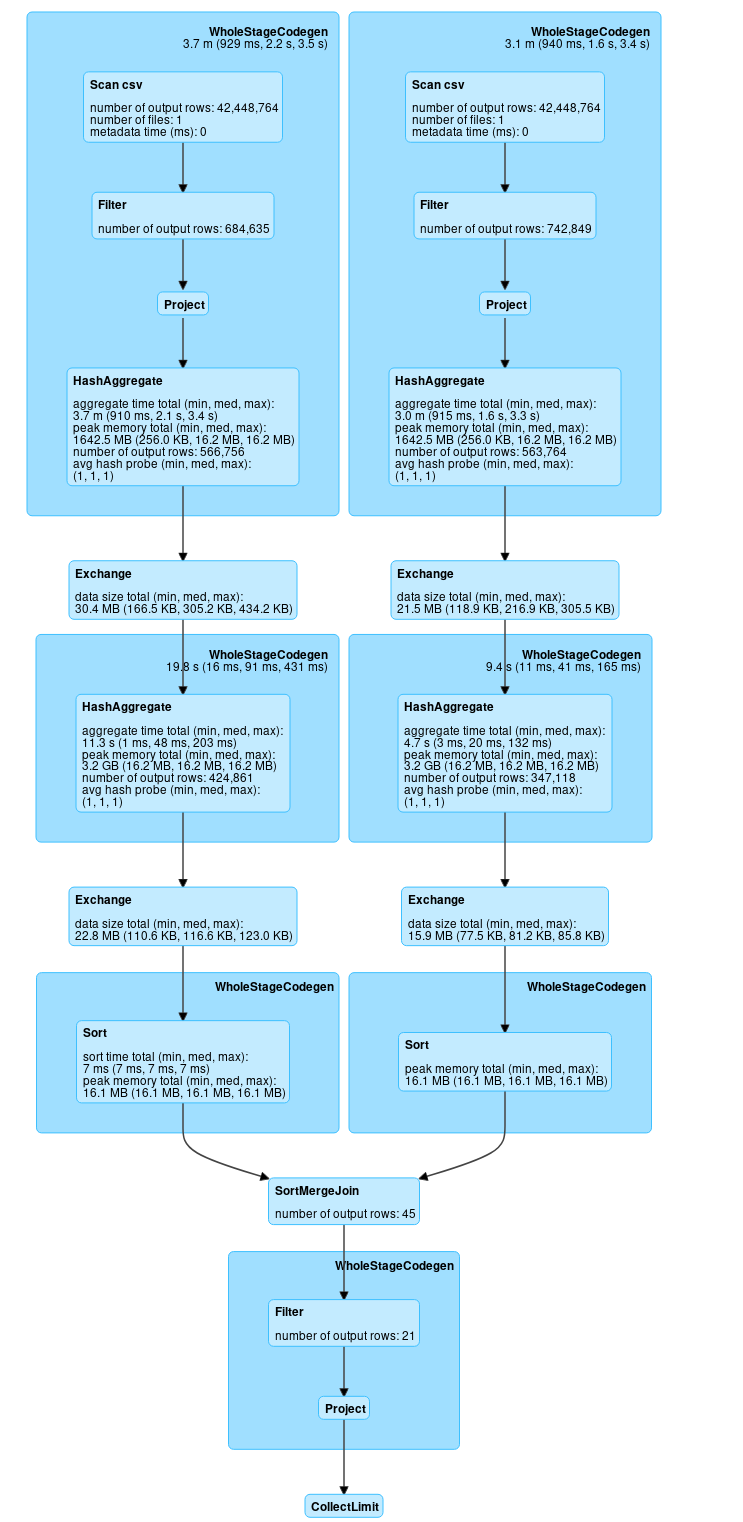
\includegraphics[width=.45\textwidth]{query3.png}
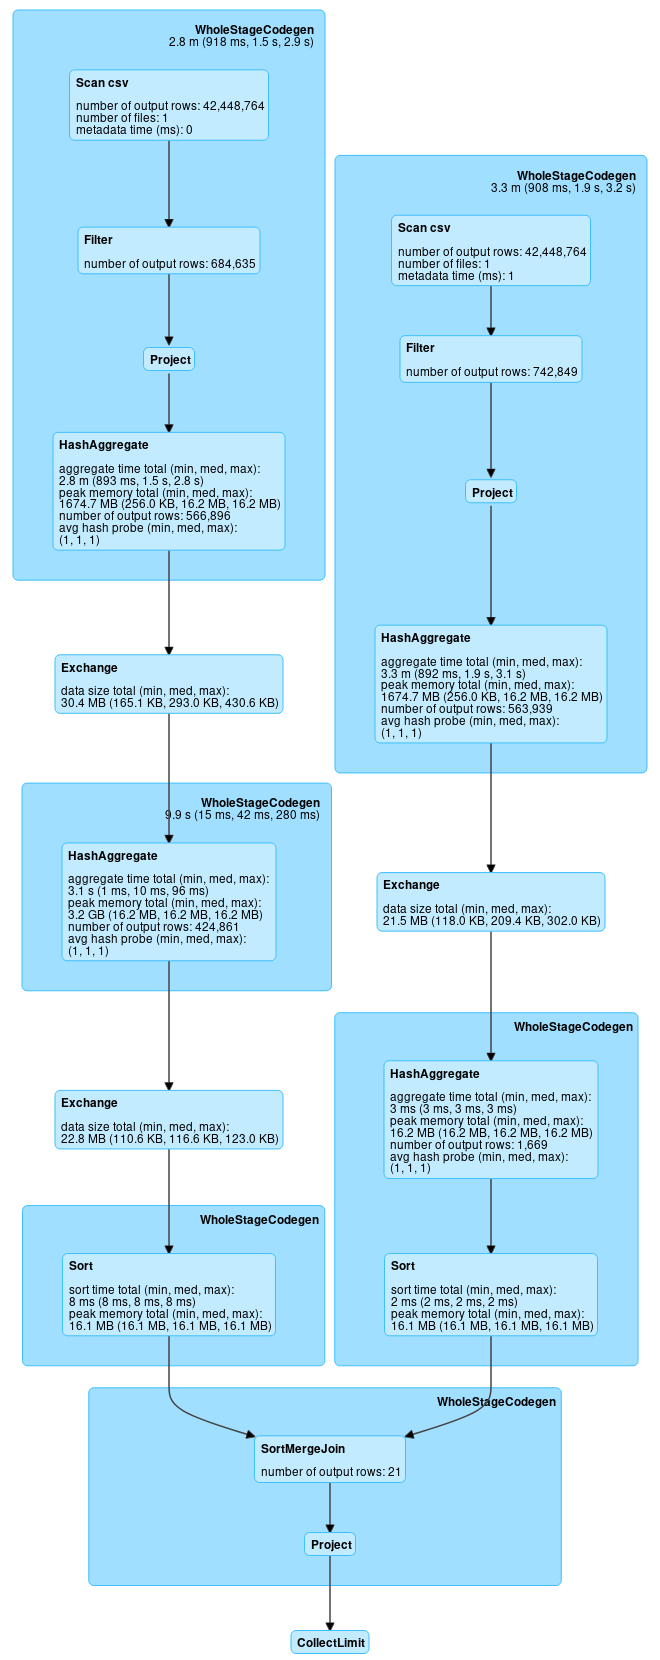
\includegraphics[width=.45\textwidth]{query32.png}
\label{fig:query3.exec}
\caption{Execution plans for \ref{it:query3}}
\end{figure}

\begin{figure}[p]
	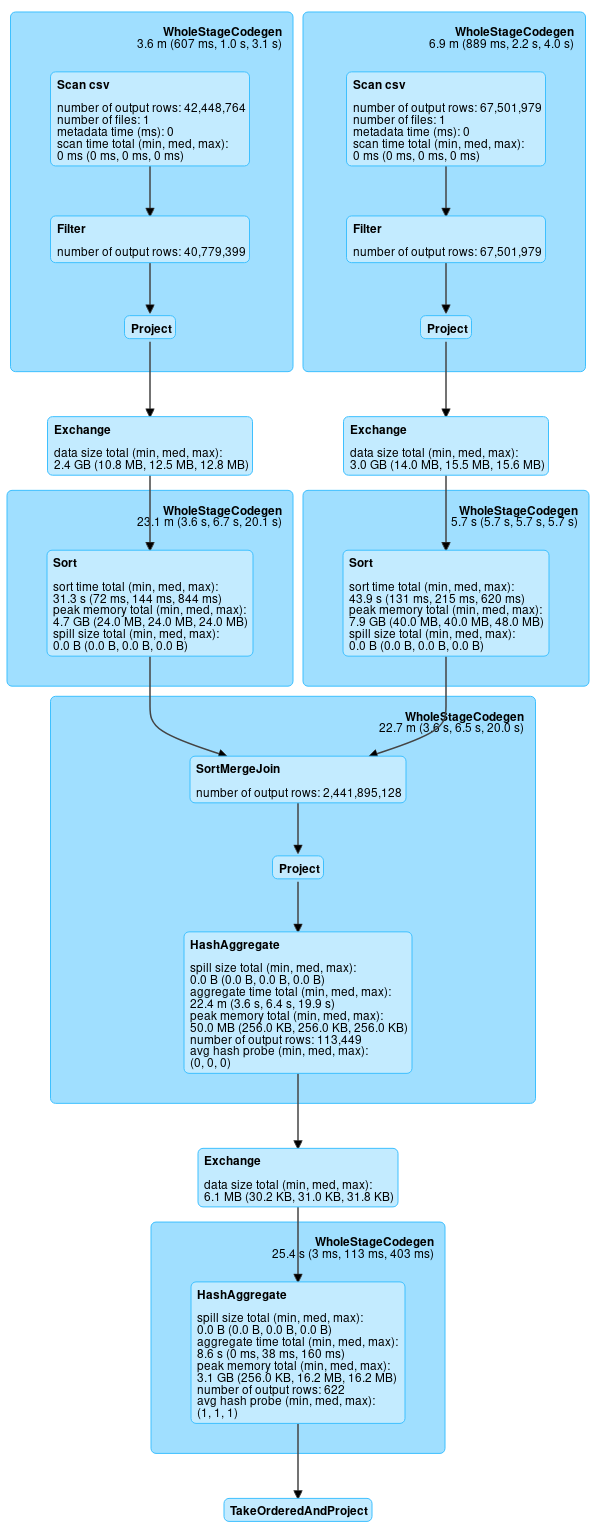
\includegraphics[width=.45\textwidth]{query4.png}
	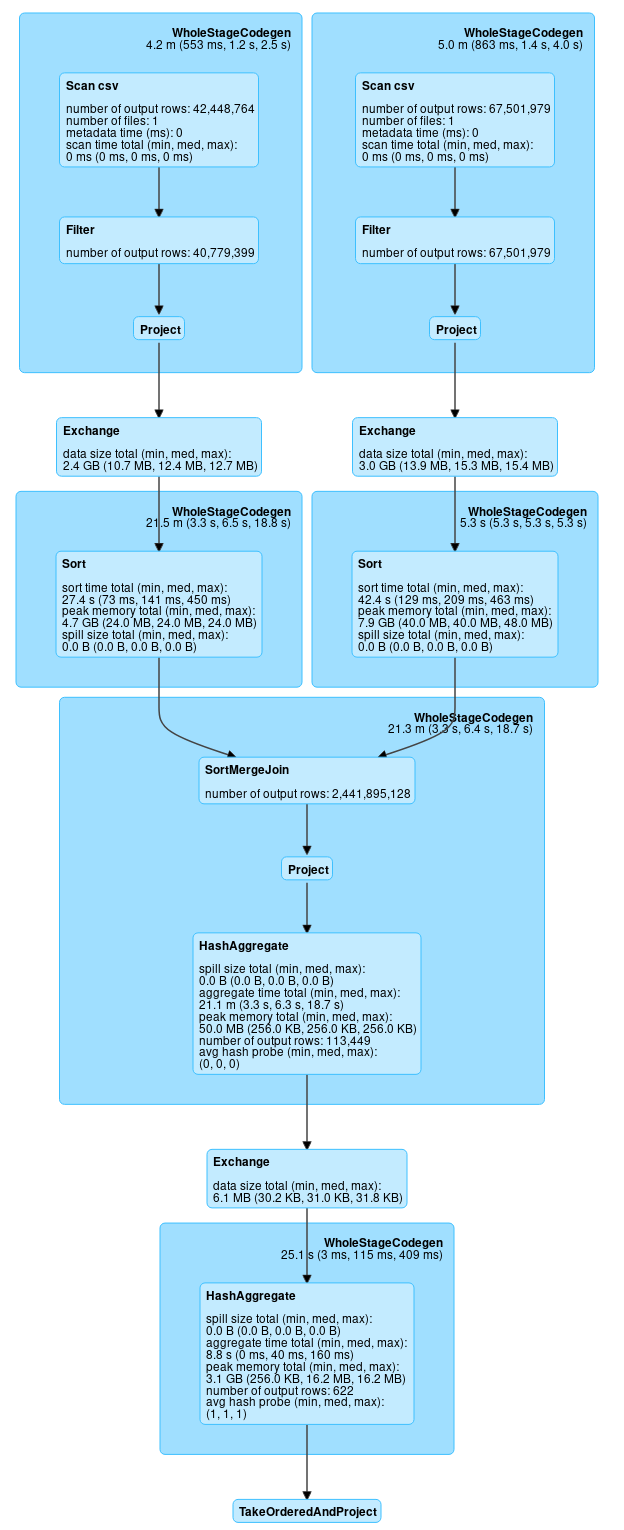
\includegraphics[width=.45\textwidth]{query42.png}
	\label{fig:query4.exec}
	\caption{Execution plans for \ref{it:query4}}
\end{figure}
  
\end{exercise}




\end{document}
